\section{Backend-Logik}\label{Sec:Backend-Logik}

Die Logik des Feasibility-Check-Algorithmus basiert auf vier zentralen Methoden, die gemeinsam die Machbarkeitsprüfung eines Tests durchführen:  

\begin{enumerate}
    \item \textbf{Helfer-Methode}: Diese Methode ruft die eigentliche \texttt{FeasibilityCheck()-Methode} auf und stellt sicher, dass der Aufrufer der REST-API eine aussagekräftige Rückmeldung erhält.  
    \item \textbf{FeasibilityCheck()-Methode}: Sie bildet die Kernkomponente und entscheidet, welche der beiden folgenden Prüfungen durchgeführt wird.  
    \item \textbf{Condition Check}: Eine eigenständige Methode zur Überprüfung der Sinnhaftigkeit der angelegten Parameter-Werte
    \item \textbf{Equipment Check}: Eine eigenständige Methode zur Überprüfung der Durchführbarkeit der angelegten Parameter-Werte
\end{enumerate}  

Der Ablauf der einzelnen Methoden wird durch jeweils ein Aktivitäts- bzw. Flussdiagramme visualisiert. In diesen Diagrammen sind Schleifen durch farblich hervorgehobene Bereiche dargestellt, die jeweils als Einstiegs- und Ausstiegspunkt gleichfarbige Kreise enthalten.


\subsection{Helfer-Methode}

Die Ausführung des Algorithmus wird initiiert, sobald der Benutzer im Frontend einen Button in der Weboberfläche betätigt. Dies löst einen asynchronen HTTP-Call über eine REST-API aus, welcher die \textbf{Helfer-Methode} aufruft und die Test-ID des zu überprüfenden Tests als Argument übergibt.

\begin{figure}[!htbp]
    \centering
    \makebox[\textwidth]{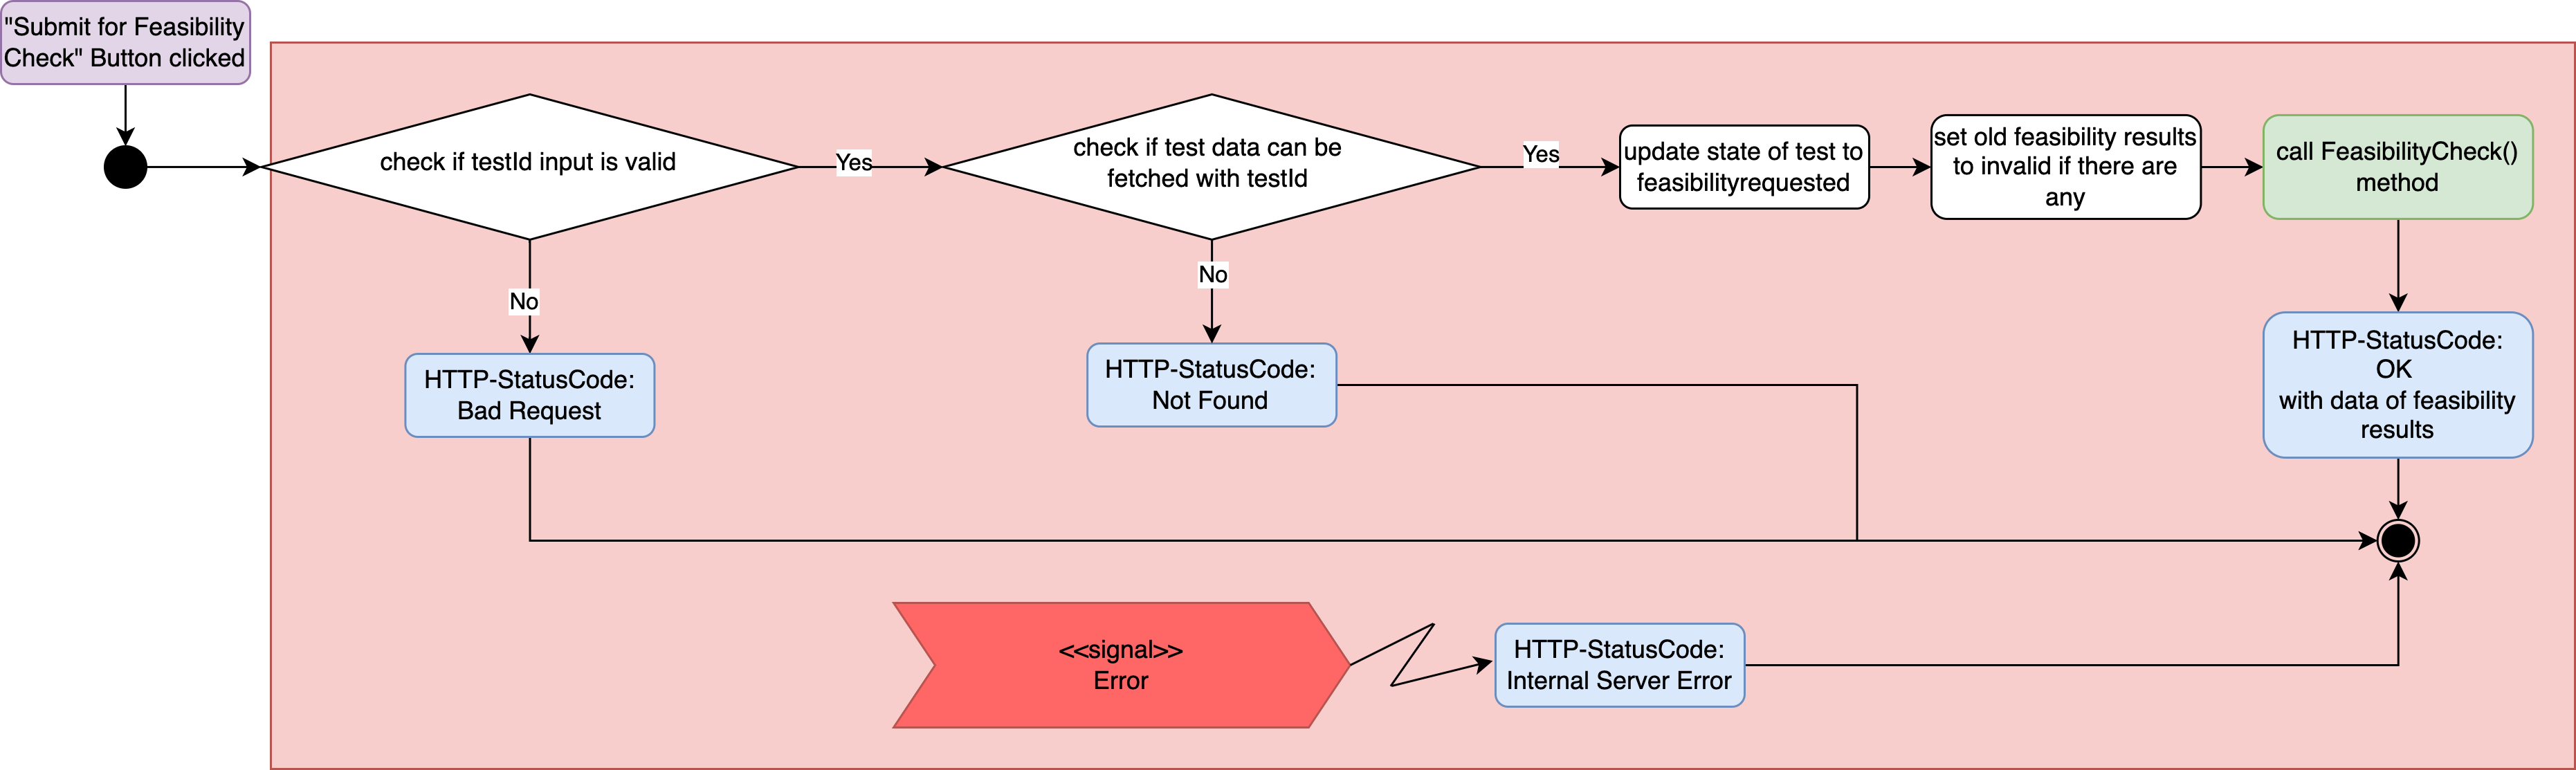
\includegraphics[width=1\textwidth]{bilder/flowchart-check-feasibility-http-call-6-2.png}}
    \caption{Flussdiagramm der Helfer-Methode}
    \label{fig:feasibility-http-call-method}
\end{figure}

Der Ablauf dieser Helfer-Methode ist in Abbildung \ref{fig:feasibility-http-call-method} dargestellt. Ihre Hauptaufgabe besteht darin, die eigentliche \texttt{FeasibilityCheck()}-Methode (grün markierte Aktivität in der Graphik \ref{fig:feasibility-http-call-method}) auszuführen und zusätzlich eine geeignete HTTP-Statusmeldung an das Frontend bzw. den Benutzer zurückzugeben. Zusätzlich wird vor der Verarbeitung die übergebene Test-ID auf Gültigkeit überprüft und der Test-Status auf ''\texttt{FEASIBILITYREQUESTED}'' aktualisiert. Falls der FeasibilityCheck für diesen Test bereits zuvor durchgeführt wurde, müssen alte Ergebnisse in der Datenbank noch als ''invalid'' markiert werden.


Zur besseren Übersicht wird in Abbildung \ref{fig:feasibility-http-call-method} auch der initiale Button-Klick im Frontend als Aktivität (lila markiert) dargestellt. Die eigentliche Logik der Methode beginnt jedoch erst nach dem schwarzen Einstiegspunkt, der den Start des Algorithmus kennzeichnet.

Zur Verbesserung der Fehlerrobustheit, wie sie in den Anforderungen definiert ist, stellt die Methode sicher, dass jede unerwartete Situation – beispielsweise ungültige Eingaben oder fehlende Testdaten – mit einem klar definierten HTTP-Status-Code beantwortet wird. So führt eine ungültige Test-ID zu einem \texttt{Bad Request} (400), während eine nicht auffindbare Test-ID mit einem \texttt{Not Found} (404) quittiert wird. Falls während der Verarbeitung interne Fehler auftreten, werden diese durch einen \texttt{Internal Server Error} (500) abgefangen. Dadurch bleibt das System auch bei unerwarteten Dateninkonsistenzen oder unvollständigen Parametern stabil und liefert stets eine eindeutige Rückmeldung an den Benutzer bzw. das aufrufende System.

\subsection{Feasibility Check}

\begin{figure}[!htbp]
    \centering
    \makebox[\textwidth]{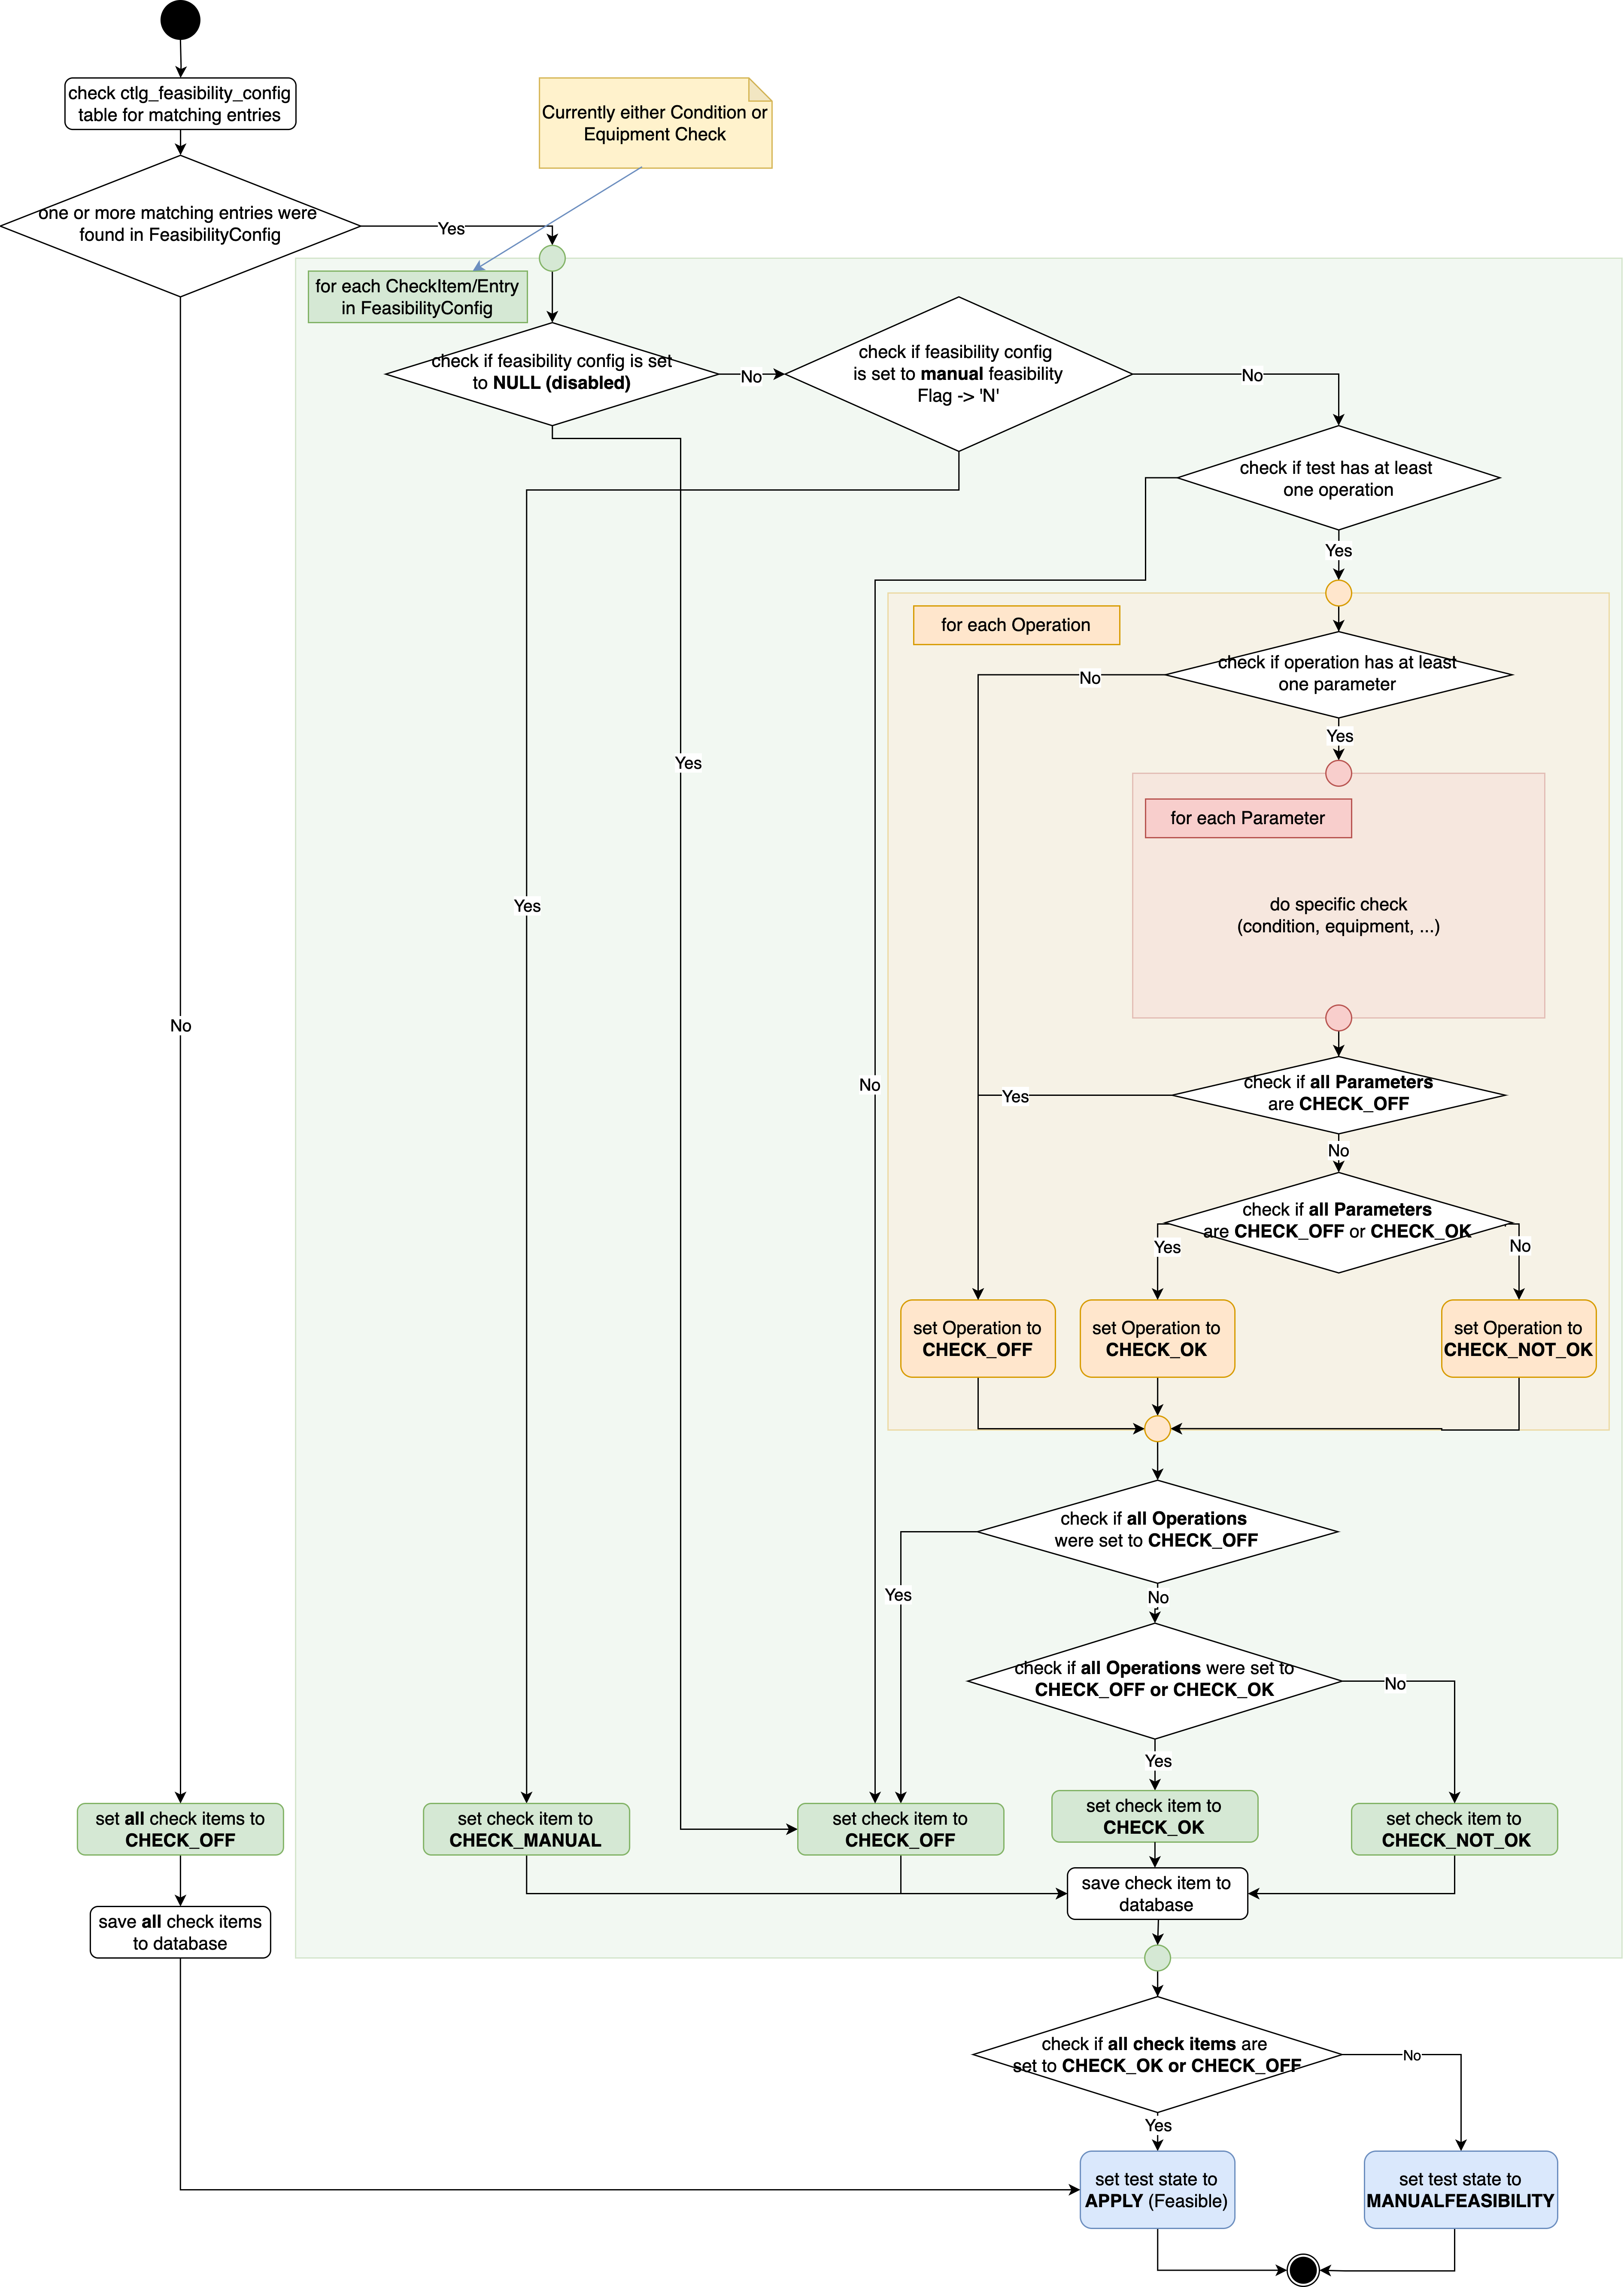
\includegraphics[width=0.85\paperwidth]{bilder/flowchart-feasibilitycheck-modiefied-for-thesis-6-2.png}}
    \caption{Flussdiagramm des Feasibility Checks}
    \label{fig:feasibility-check}
\end{figure}

Die Kernlogik des Feasibility Checks wird durch die Methode \textbf{\texttt{FeasibilityCheck()}} ausgeführt, die im Flussdiagramm in Abbildung \ref{fig:feasibility-check} detailliert dargestellt ist. Diese Methode erhält von der Helfer-Methode die Test-ID und überprüft die \textit{Feasibility} des Tests anhand der relevanten Parameter und Operationen. Um die Logik des Algorithmus zu vereinfachen, wird eine Statustyp-Klasse (\textit{Enum}) eingeführt, die den Endstatus einzelner \textit{Feasibility-Teil-Checks} kennzeichnet. Dieser besteht aus vier möglichen Zuständen, deren jeweilige Bedeutungen in Tabelle \ref{tab:feasibility-states} erläutert werden.

\begin{table}[!htb]
    \centering
    \caption{(End-)Status von Feasibility-Teil-Checks, gespeichert als \texttt{FCIR\_STATE} in Feasibility Result (\texttt{feasibility\_check\_item\_result})}
    \footnotesize
    \renewcommand{\arraystretch}{1.3} % Erhöht den Zeilenabstand
    \begin{tabular}{p{0.25\linewidth} p{0.7\linewidth}}
        \toprule
        \textbf{(End-)Status} & \textbf{Beschreibung} \\
        \midrule
        \texttt{CHECK\_OFF} & Der Check ist deaktiviert; eine Überprüfung ist weder erforderlich noch vorgesehen. Dies ist insbesondere der Fall, wenn ein Parameter bzw. eine Operation keine Stressoperation darstellt und somit kein Parameter-Wert (PlanValue) definiert werden muss. \\
        \midrule
        \texttt{CHECK\_OK} & Der Check war erfolgreich. \\
        \midrule
        \texttt{CHECK\_NOT\_OK} & Der Check war nicht erfolgreich oder es ist ein Fehler aufgetreten. \\
        \midrule
        \texttt{CHECK\_MANUAL} & Eine automatische Überprüfung ist nicht möglich oder der Check ist noch nicht für die automatisierte Überprüfung zugelassen; der Check muss von einem Mitarbeiter manuell durchgeführt werden. \\
        \bottomrule
    \end{tabular}
    \label{tab:feasibility-states}
\end{table}

Jede zu überprüfende Einheit – sei es auf Parameter-, Operations- oder CheckItem-Ebene (Condition oder Equipment Check) – wird individuell bewertet und erhält einen entsprechenden Status. Der Algorithmus arbeitet hierarchisch: Zunächst erfolgt die Bewertung auf der untersten Ebene, also bei den Parametern, sofern diese vorhanden sind. Sind Operationen enthalten, werden diese sowie deren zugehörige Parameter einzeln geprüft, wobei für jeden Parameter, der ein prüfbares Ergebnis liefert, ein Feasibility-Ergebnis in der Datenbank abgelegt wird. Falls ein Test zwar Operationen enthält, diese jedoch keine Parameter vorweisen, erfolgt die Speicherung ausschließlich auf der Ebene der Operation. Liegen überhaupt keine Operationen vor, wird lediglich ein Gesamtergebnis für den Test erfasst.

Obwohl die Ergebnisse der untergeordneten Ebenen zu einem Gesamtstatus aggregiert werden – beispielsweise durch die Zusammenfassung der Parameter-Resultate zu einem Operations-Ergebnis (siehe orange markierte Aktivitäten in Abb. \ref{fig:feasibility-check}) und der Operations-Ergebnisse zu einem CheckItem-Ergebnis (sei es ein \gls{ConditionCheck} oder \gls{EquipmentCheck}, dargestellt in den grünen Aktionen) – wird in der Datenbank ausschließlich das Resultat der jeweils untersten vorhandenen Ebene persistent abgelegt. Durch diese Maßnahme in Kombination mit der bewussten Nicht-Speicherung von Ergebnissen, die lediglich den Status \texttt{CHECK\_OFF} aufweisen, wird eine unnötige Datenbankaufblähung vermieden und die Systembelastung reduziert, da diese Ergebnisse keine zusätzlichen, nutzerrelevanten Informationen liefern. Zudem wird der Persistierungsvorgang in den Flussdiagrammen nicht explizit dargestellt, da die Speicherung auf unterschiedlichen Ebenen erfolgt und eine detaillierte Visualisierung die Diagramme erheblich komplexer machen würde.

Basierend auf den Ergebnissen aller CheckItems wird schließlich der finale Test-Status bestimmt. Dieser kann entweder den Wert \textbf{''APPLY''} (''Feasible'', also erfolgreich) oder \textbf{''MANUALFEASIBILITY''} (manuelle Prüfung erforderlich) (blau markierte Aktivitäten in Abb. \ref{fig:feasibility-check}) annehmen.

Für Tests bei denen die relevante Feasibililty-Konfigurationstabelle leer ist oder das CheckItem auf \textit{null} steht, wertet das System die (Teil-)Überprüfung als \texttt{CHECK\_OFF} und somit indirekt als erfolgreich, weil keine Prüfung erforderlich ist.

\textbf{Konkreter Ablauf des Feasibility Check Algorithmus} \\
Zunächst werden die für den Test hinterlegten Konfigurationen für jedes CheckItem aus der Datenbank abgerufen. Falls kein Eintrag existiert, wird der Check automatisch als erfolgreich gewertet. Ist das zugehörige Flag auf 'N' gesetzt, muss die Überprüfung manuell erfolgen, und der Check ist an dieser Stelle beendet. Nur wenn das Flag auf 'Y' gesetzt ist, wird das entsprechende CheckItem (Condition oder \gls{EquipmentCheck}) tatsächlich geprüft.

Anschließend wird kontrolliert, ob der Test mindestens eine Operation enthält. Falls dies der Fall ist, wird jede Operation einzeln überprüft, um festzustellen, ob sie keinen, einen oder mehrere Parameter besitzt. Für jeden dieser Parameter wird dann der entsprechende \gls{ConditionCheck} oder \gls{EquipmentCheck} durchgeführt. Welche der beiden Prüfungen erfolgt, hängt vom jeweiligen CheckItem ab. Die genaue Funktionsweise dieser Methoden wird in den folgenden Kapiteln erläutert.

Durch diese Struktur ist das System nicht nur auf die aktuellen CheckItem-Typen beschränkt, sondern kann zukünftig um weitere Prüfmethoden erweitert werden. Neue Checks lassen sich problemlos integrieren, ohne den bestehenden Ablauf grundlegend ändern zu müssen. Dies gewährleistet die in den Anforderungen definierte Flexibilität und modulare Erweiterbarkeit des Systems (siehe Kapitel \ref{Sec:funktionale-anforderungen}).

\subsection{Condition Check}
\begin{figure}[!htb]
    \centering
    \makebox[\textwidth]{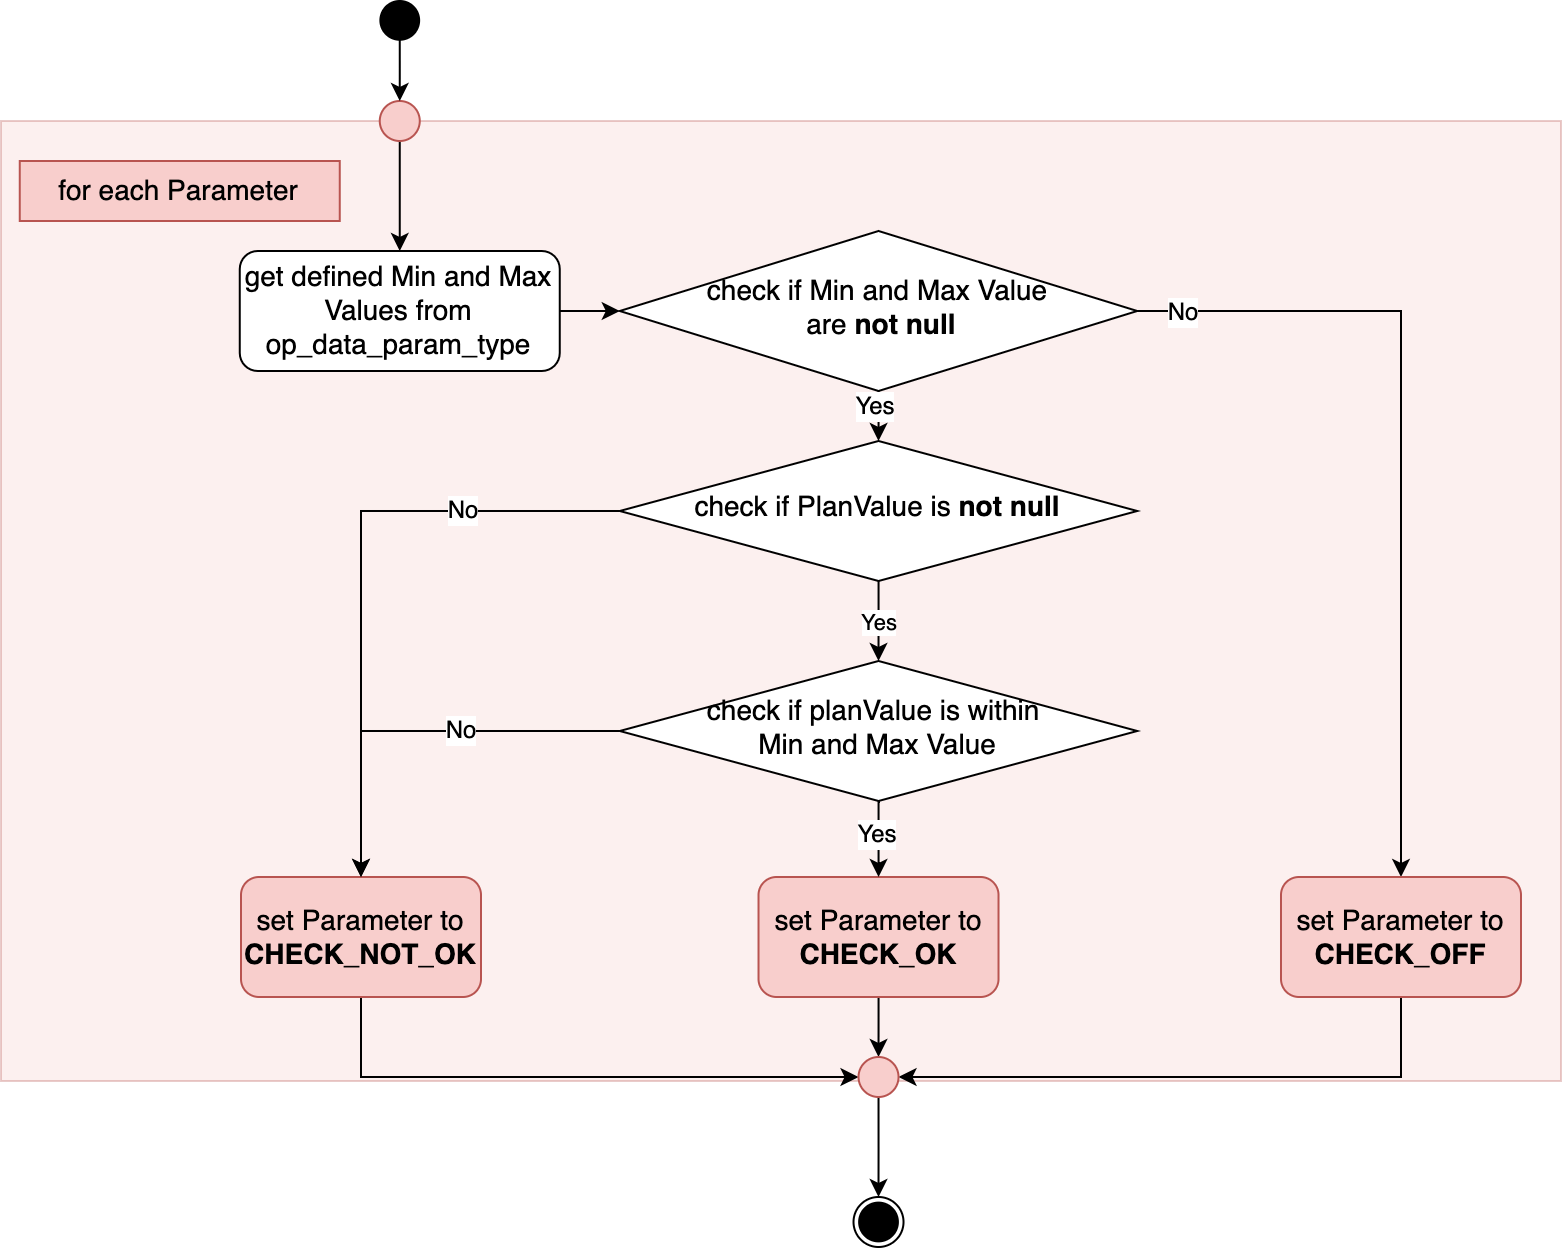
\includegraphics[width=0.80\paperwidth]{bilder/flowchart-condition-check-6-2.png}}
    \caption{Flussdiagramm des \gls{ConditionCheck}s}
    \label{fig:condition-check}
\end{figure}

Der Ablauf des \gls{ConditionCheck} ist in Abbildung \ref{fig:condition-check} dargestellt. Zunächst wird die relevante Verknüpfungstabelle \texttt{op\_data\_param\_type} aus der Datenbank ausgelesen. Diese Tabelle definiert den zulässigen Wertebereich eines Parameters, durch einen minimalen und maximalen Wert in den neu eingefügten Spalten (\texttt{OPT\_CD\_MIN} und \texttt{OPT\_CD\_MAX}). Falls keiner der beiden Wert definiert ist, wird der \textit{Parameter-Teil-Check} auf \texttt{CHECK\_OFF} gesetzt, was bedeutet, dass keine Überprüfung erforderlich ist und der Parameter automatisch als gültig betrachtet wird. Sind sowohl ein minimaler als auch ein maximaler Wert hinterlegt, muss zusätzlich ein geplanter Wert (PlanValue) für den Parameter vorhanden sein. Liegt dieser innerhalb des zulässigen Bereichs, gilt die Sinnhaftigkeitsprüfung als erfolgreich, und der nächste Parameter der Operation wird verarbeitet. 

In Sonderfällen, in denen lediglich ein Mindest- oder Höchstwert vorliegt, genügt es, wenn der PlanValue die entsprechende Bedingung (über dem Mindestwert oder unter dem Höchstwert) erfüllt – diese Fälle sind im Flussdiagramm zur besseren Übersichtlichkeit nicht dargestellt.


\subsection{Equipment Check}

\begin{figure}[!htbp]
    \centering
    \makebox[\textwidth]{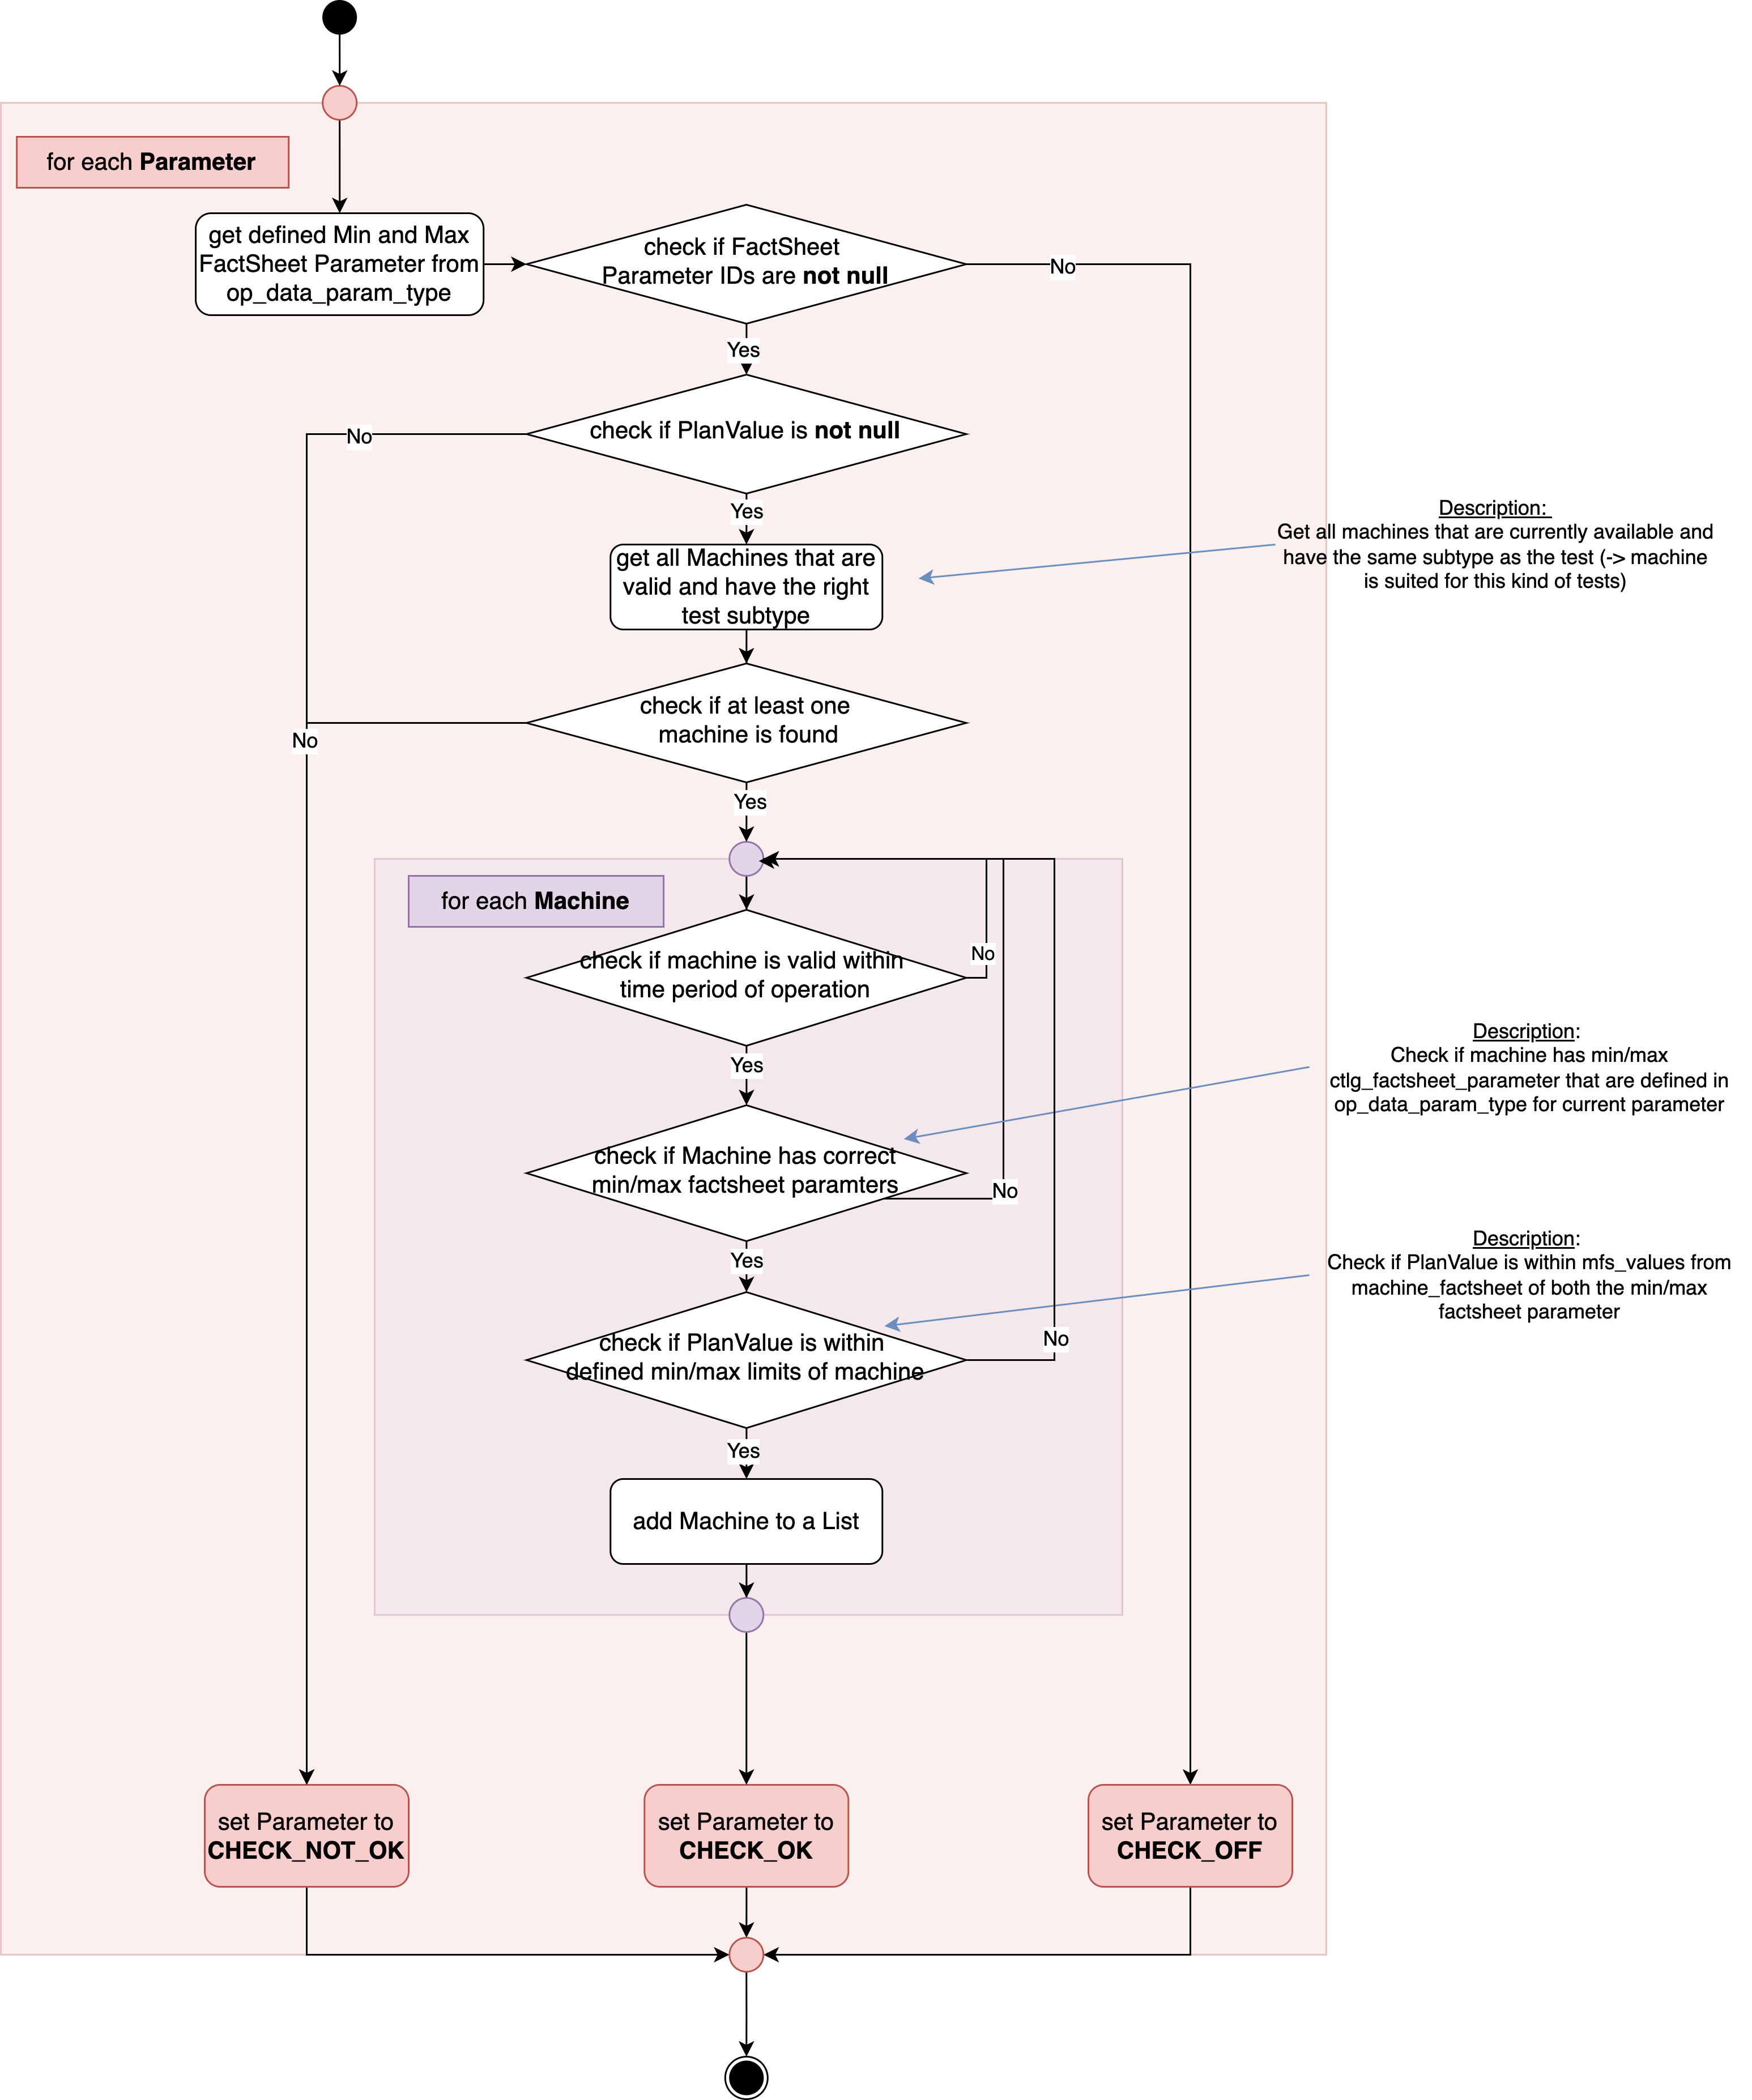
\includegraphics[width=0.85\paperwidth]{bilder/flowchart-equipment-check-6-2.png}}
    \caption{Flussdiagramm des \gls{EquipmentCheck}s}
    \label{fig:equipment-check}
\end{figure}

Der \gls{EquipmentCheck} ist in Abbildung \ref{fig:equipment-check} dargestellt. Der Prozess beginnt ebenfalls mit dem Abruf von Daten aus der passenden \texttt{op\_data\_param\_type} Tabelle. Falls keine Referenzen für den minimalen und maximalen Maschinen-Parameter (\texttt{ctlg\_\-factsheet\_\-parameter}) hinterlegt sind, ist die Überprüfung für diesen (Operations-)\-Parameter, nicht erforderlich und ist somit beendet. Andernfalls muss sichergestellt werden, dass ein PlanValue gesetzt ist. Erst danach startet der eigentliche Durchführbarkeits-Check.

Als Erstes werden aus der Datenbank alle Maschinen abgerufen, die als ''valide'' gelten, also weder defekt noch in Wartung sind und zudem den gleichen Test-Typen aufweisen wie der zu prüfende Test. Die Zuordnung der Maschinen zu einem spezifischen Test-Typen erfolgt dabei indirekt über die Verknüpfungstabelle \texttt{machine\_\-test\_\-sub\_type}, welche die Maschinen mit dem jeweiligen \texttt{ctlg\_test\_sub\_type} verknüpft.

Anschließend werden die verbleibenden Maschinen einzeln durchlaufen (siehe lila markierter Bereich in Abbildung \ref{fig:equipment-check}). Zuerst wird analysiert, ob die Maschine im geplanten Zeitraum der Operation zur Verfügung steht. Danach erfolgt die Überprüfung, ob die Maschine den Parameter grundsätzlich umsetzen kann. Dazu wird geprüft, ob die Maschine über die gleichen \texttt{ctlg\_factsheet\_parameter} verfügt, die in der Verknüpfungstabelle definiert sind. Falls dies der Fall ist, werden die minimalen und maximalen Werte über den zugehörigen Eintrag im Maschinen-Factsheet (\texttt{MFS\_VALUE}) ausgelesen. Anschließend wird kontrolliert, ob der geplante Wert (\textit{PlanValue}) des Parameters innerhalb dieser Grenzen liegt. Ist dies der Fall, gilt die Maschine als geeignet, den geplanten Wert umzusetzen. 

Wird mindestens eine Maschine gefunden, wird der \gls{EquipmentCheck} für diesen Parameter als erfolgreich betrachtet. Zudem werden alle Maschinen, die den Parameter mit dem geplanten Wert umsetzen können, in einer Liste als \texttt{check\_item\_result\_\-list} erfasst und mit dem zugehörigen \texttt{feasibility\_check\_item\_result} in der Datenbank abgespeichert.


\subsection{Benutzer Feedback}\label{Subsec:user-feedback}

Damit der Endnutzer das Ergebnis des Feasibility Checks nachvollziehen kann, wird jedem Feasibility-Resultat in der Datenbank eine spezifische, nutzerfreundliche Erklärung zugeordnet (\texttt{FCIR\_DESCRIPTION}). Diese Rückmeldungen sind nach den unterschiedlichen Überprüfungsebenen (Test, Operation, Parameter) strukturiert, sodass der Benutzer präzise erkennen kann, an welcher Stelle Handlungsbedarf besteht. In folgenden Tabellen \ref{tab:feedback-test}, \ref{tab:feedback-operation}, \ref{tab:feedback-condition} und \ref{tab:feedback-equipment} werden die wichtigsten Rückmeldungen dargestellt.

Feasibility-Results mit dem Status \texttt{CHECK\_OFF} werden im Regelfall nicht gespeichert, da sie keine zusätzlichen, für den Benutzer relevanten Informationen liefern. Die Abspeicherung dieser Ergebnisse kann jedoch zu Debugging-Zwecken temporär aktiviert werden, um eine detailliertere Analyse der Prüfschritte zu ermöglichen.


\begin{table}[!htb]
    \centering
    \caption{Feedback auf Test-Ebene}
    \footnotesize
    \renewcommand{\arraystretch}{1.1} % Erhöht den Zeilenabstand
    \setlength{\arrayrulewidth}{0.1pt} % Dünnere Linien
    \begin{tabular}{p{0.8\linewidth} p{0.15\linewidth}}
        \textbf{Meldung} & \textbf{Status} \\
        \midrule
        Feasibility Configuration not found & \texttt{CHECK\_OFF} \\
        \midrule
        Check Item is disabled for automatic feasibility check, see \texttt{ctlg\_feasibillity\_config} & \texttt{CHECK\_MANUAL} \\
        \midrule
        No Operations found for this test & \texttt{CHECK\_OFF} \\
        \bottomrule
    \end{tabular}
    \label{tab:feedback-test}
\end{table}


\begin{table}[!htb]
    \centering
    \caption{Feedback auf Operations-Ebene}
    \footnotesize
    \renewcommand{\arraystretch}{1.1}
    \begin{tabular}{p{0.8\linewidth} p{0.15\linewidth}}
        \textbf{Meldung} & \textbf{Status} \\
        \midrule
        Operation with no Parameters & \texttt{CHECK\_OFF} \\
        \bottomrule
    \end{tabular}
    \label{tab:feedback-operation}
\end{table}


\begin{table}[!htb]
    \centering
    \caption{Feedback auf Parameter-Ebene -- Condition Check}
    \footnotesize
    \renewcommand{\arraystretch}{1.1}
    \begin{tabular}{p{0.8\linewidth} p{0.15\linewidth}}
        \textbf{Meldung} & \textbf{Status} \\
        \midrule
        No \texttt{op\_data\_param\_type} was found for this parameter & \texttt{CHECK\_NOT\_OK} \\
        \midrule
        No Conditions defined & \texttt{CHECK\_OFF} \\
        \midrule
        Error: PlanValue is not set & \texttt{CHECK\_NOT\_OK} \\
        \midrule
        Check successful: PlanValue=\{\textit{planValue}\}, ConditionMin=\{\textit{ConditionMin}\}, ConditionMax=\{\textit{ConditionMax}\} & \texttt{CHECK\_OK} \\
        \midrule
        Check failed: PlanValue=\{\textit{planValue}\}, ConditionMin=\{\textit{ConditionMin}\}, ConditionMax=\{\textit{ConditionMax}\} & \texttt{CHECK\_NOT\_OK} \\
        \bottomrule
    \end{tabular}
    \label{tab:feedback-condition}
\end{table}


\begin{table}[!htb]
    \centering
    \caption{Feedback auf Parameter-Ebene -- Equipment Check}
    \footnotesize
    \renewcommand{\arraystretch}{1.1}
    \begin{tabular}{p{0.8\linewidth} p{0.15\linewidth}}
        \textbf{Meldung} & \textbf{Status} \\
        \midrule
        No \texttt{op\_data\_param\_type} was found for this parameter & \texttt{CHECK\_NOT\_OK} \\
        \midrule
        No Equipment Parameters defined & \texttt{CHECK\_OFF} \\
        \midrule
        Error: PlanValue is not set & \texttt{CHECK\_NOT\_OK} \\
        \midrule
        Check failed: Found no valid machines with Testsubtype of Test & \texttt{CHECK\_NOT\_OK} \\
        \midrule
        Check successful: Found \{\textit{numberOfMachines}\} Machines for: PlanValue=\{\textit{planValue}\}, EquipmentParameterMin=\{\textit{ParameterMin}\}, EquipmentParameterMax=\{\textit{ParameterMax}\} & \texttt{CHECK\_OK} \\
        \midrule
        Check failed: Found no Machines: ... & \texttt{CHECK\_NOT\_OK} \\
        \quad Reason: Found no valid Machine within time period ... & \\
        \quad Reason: Found no valid Machine with needed Parameters ... & \\
        \quad Reason: Current PlanValue=\{\textit{planValue}\} too high: Please set PlanValue lower & \\
        \quad Reason: Current PlanValue=\{\textit{planValue}\} too low: Please set PlanValue higher & \\
        \bottomrule
    \end{tabular}
    \label{tab:feedback-equipment}
\end{table}



Die dargestellten Rückmeldungen ermöglichen es dem Benutzer, gezielt auf vom Feasibility Check-Alorithmus erkannte Probleme zu reagieren. So kann er beispielsweise den PlanValue anpassen, wenn darauf hingewiesen wird, dass der aktuelle Wert zu hoch oder zu niedrig ist, wie in Tabelle~\ref{tab:feedback-equipment} unten dargestellt. Diese detaillierten Informationen unterstützten den Benutzer bei der Identifikation und Behebung von Konfigurationsproblemen. 

Dadurch erfüllt das Feedback eine zentrale funktionale Anforderung (siehe Kapitel \ref{Sec:funktionale-anforderungen}) an den automatisierten Feasibility Check: die Nachvollziehbarkeit der Ergebnisse. Anstelle einer einfachen „Ja/Nein“-Bewertung erhält der Benutzer eine transparente Begründung der Entscheidung, wodurch unerwartete Probleme besser analysiert und die Test-Parameter gezielt optimiert werden können.